\chapter{Library Design}

A major challenge which arises when one aims to develop a software package that
implements the spectral/hp element method is to implement the mathematical
structure of the method in a digestible and coherent matter. Obviously, there
are many ways to encapsulate the fundamental concepts related to the
spectral/$hp$ element method, depending on e.g. the intended goal of the
developer or the chosen programming language. We will (without going in too much
detail) give a an overview of how we have chosen to abstract and implement
spectral/hp elements in the \nekpp library. However, we want to emphasise that
this is not the only possible choice.

Five different sublibraries, employing this characteristic pattern, are provided
in the full \nekpp library:

\begin{itemize}
\item the standard elemental region sublibrary (StdRegions library)
\item the parametric mapping sublibrary (SpatialDomains library)
\item the local elemental region sublibrary (LocalRegions library)
\item the global region sublibrary (MultiRegions library)
\item the supporting utilities sublibrary (LibUtilities library)
\end{itemize}

This structure can also be related to the formulation of a global spectral/hp
element expansion, i.e.

\begin{align*}
  u(\boldsymbol{x})=\overbrace{\sum_{e\in\mathcal{E}}\underbrace{\sum_{n\in\mathcal{N}}\phi^e_n(\boldsymbol{x})\hat{u}^e_n}_{\mbox{\scriptsize{LocalRegions
  library}}}}^{\mbox{\scriptsize{MultiRegions
  library}}}=\sum_{e\in\mathcal{E}}\underbrace{\sum_{n\in\mathcal{N}}\phi^{std}_n\overbrace{(\left[\chi^e\right]^{-1}(\boldsymbol{x}))}^{\mbox{\scriptsize{SpatialDomains
  library}}}\hat{u}^e_n}_{\mbox{\scriptsize{StdRegions library}}}
\end{align*}

A more detailed overview of the \nekpp structure, including an overview of
the most important classes per sublibrary, is depicted in the
Figure~\ref{f:library:overview}.

\begin{figure}
\centering
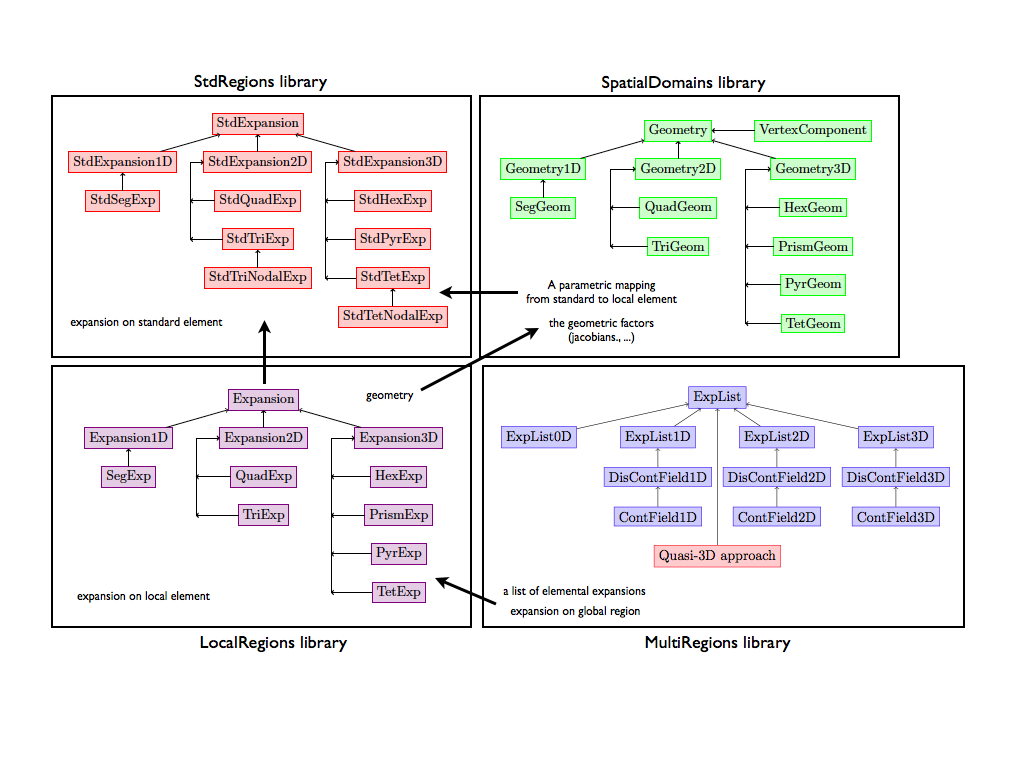
\includegraphics[width=\textwidth]{img/overview.png}
\caption{Diagram of the important classes in each library.}
\label{f:library:overview}
\end{figure}

\section{LibUtilities}

This contains the underlying building blocks for constructing a spectral element
formulation including linear algebra, polynomial routines and memory management
\cite{Ga39,AbSt64,CaHuYoQu88,GhOs70,KaSh05}. This includes:
\begin{itemize}
\setlength{\itemsep}{0em}
\item Basic Constants
\item Basic Utilities ( Nektar++ Arrays)
\item Expression Templates
\item Foundations
\item Interpreter
\item Kernel
\item Linear Algebra
\item Memory Management
\item Nodal Data
\item Polynomial Subroutines
\item Time Integration
\end{itemize}

\subsection{The Polylib library}
These are routines for orthogonal polynomial calculus and interpolation based on
codes by Einar Ronquist and Ron Henderson.

\subsubsection{Abbreviations}
\begin{tabular}{ll}
\toprule
Character(s) & Description \\
\midrule
z & Set of collocation/quadrature points \\
w & Set of quadrature weights \\
D & Derivative matrix \\
h & Lagrange Interpolant \\
I & Interpolation matrix \\
g & Gauss \\
k & Kronrod \\
gr & Gauss-Radau \\
gl & Gauss-Lobatto \\
j & Jacobi \\
m & point at minus 1 in Radau rules \\
p & point at plus 1 in Radau rules \\
\bottomrule
\end{tabular}


\subsubsection{Main routines}
\begin{tabular}{ll}
\toprule
\multicolumn{2}{l}{\textbf{Points and Weights}} \\
Routine & Description \\
\midrule
zwgj & Compute Gauss-Jacobi points and weights \\
zwgrjm & Compute Gauss-Radau-Jacobi points and weights (z=-1) \\
zwgrjp & Compute Gauss-Radau-Jacobi points and weights (z= 1) \\
zwglj & Compute Gauss-Lobatto-Jacobi points and weights \\
zwgk & Compute Gauss-Kronrod-Jacobi points and weights \\
zwrk & Compute Radau-Kronrod points and weights \\
zwlk & Compute Lobatto-Kronrod points and weights \\
JacZeros & Compute Gauss-Jacobi points and weights \\
\bottomrule
\end{tabular}

\begin{tabular}{ll}
\toprule
\multicolumn{2}{l}{\textbf{Derivative Matrices}} \\
Routine & Description \\
\midrule
Dgj & Compute Gauss-Jacobi derivative matrix \\
Dgrjm & Compute Gauss-Radau-Jacobi derivative matrix (z=-1) \\
Dgrjp & Compute Gauss-Radau-Jacobi derivative matrix (z= 1) \\
Dglj & Compute Gauss-Lobatto-Jacobi derivative matrix \\
\bottomrule
\end{tabular}

\begin{tabular}{ll}
\toprule
\multicolumn{2}{l}{\textbf{Lagrange Interpolants}} \\
Routine & Description \\
\midrule
hgj & Compute Gauss-Jacobi Lagrange interpolants \\
hgrjm & Compute Gauss-Radau-Jacobi Lagrange interpolants (z=-1) \\
hgrjp & Compute Gauss-Radau-Jacobi Lagrange interpolants (z= 1) \\
hglj & Compute Gauss-Lobatto-Jacobi Lagrange interpolants \\
\bottomrule
\end{tabular}

\begin{tabular}{ll}
\toprule
\multicolumn{2}{l}{\textbf{Interpolation Operators}} \\
Routine & Description \\
\midrule
Imgj & Compute interpolation operator gj->m \\
Imgrjm & Compute interpolation operator grj->m (z=-1) \\
Imgrjp & Compute interpolation operator grj->m (z= 1) \\
Imglj & Compute interpolation operator glj->m \\
\bottomrule
\end{tabular}

\begin{tabular}{ll}
\toprule
\multicolumn{2}{l}{\textbf{Polynomial Evaluation}} \\
Routine & Description \\
\midrule
jacobfd & Returns value and derivative of Jacobi poly. at point z \\
jacobd & Returns derivative of Jacobi poly. at point z (valid at z=-1,1) \\
\bottomrule
\end{tabular}

\subsubsection{Local routines}
\begin{tabular}{ll}
\toprule
Routine & Description \\
\midrule
jacobz & Returns Jacobi polynomial zeros \\
gammaf & Gamma function for integer values and halves \\
RecCoeff & Calculates the recurrence coefficients for orthogonal poly \\
TriQL & QL algorithm for symmetrix tridiagonal matrix \\
JKMatrix & Generates the Jacobi-Kronrod matrix \\
\bottomrule
\end{tabular}

\subsubsection{Notes}
\begin{itemize}
\setlength{\itemsep}{0em}
\item Legendre polynomial $\alpha = \beta = 0$
\item Chebychev polynomial $\alpha = \beta = -0.5$
\item All routines are double precision.
\item All array subscripts start from zero, i.e. vector $0..N-1$
\end{itemize}



\section{StdRegions}
The StdRegions library, a summary of which is shown in
Figure~\ref{f:library:stdregions}, bundles all classes that mimic a
spectral/$hp$ element expansion on a standard region. Such an expansion, i.e.
\begin{align*}
u(\boldsymbol{\xi}_i) =
  \sum_{n\in\mathcal{N}}\phi_n(\boldsymbol{\xi}_i)\hat{u}_n,
\end{align*}
can be encapsulated in a class that essentially should only contain three data
structures, respectively representing:

\begin{itemize}
\item the coefficient vector $\hat{\boldsymbol{u}}$,
\item the discrete basis matrix $\boldsymbol{B}$, and
\item the vector $\boldsymbol{u}$ which represents the value of the expansion
at the quadrature points $\boldsymbol{\xi}_i$.
\end{itemize}

All standard expansions, independent of the dimensionality or shape of the
standard region, can be abstracted in a similar way. Therefore, it is possible
to define these data structures in an \emph{abstract} base class, i.e. the class
!StdExpansion. This base class can also contain the implementation of methods
that are identical across all shapes. Derived from this base class is another
level of abstraction, i.e. the abstract classes StdExpansion1D, StdExpansion2D
and StdExpansion3D. All other shape-specific classes (such as e.g. StdSegExp or
StdQuadExp) are inherited from these abstract base classes. These shape-specific
classes are the classes from which objects will be instantiated.
They also contain the shape-specific implementation for operations such as
integration or differentiation.

\begin{figure}
\centering
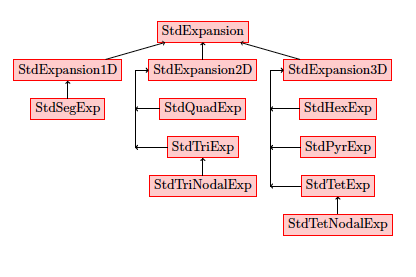
\includegraphics[width=\textwidth]{img/StdRegions.png}
\caption{Main classes in the StdRegions library.}
\label{f:library:stdregions}
\end{figure}

\section{SpatialDomains}
The most important family of classes in the SpatialDomains library is the
Geometry family, as can also be seen in Figure~\ref{f:library:spatialdomains}.
These classes are the representation of a (geometric) element in \emph{physical
space}. It has been indicated before that every local element can be considered
as an image of the standard element where the corresponding one-to-one mapping
can be represented as an elemental standard spectral/hp expansion. As such, a
proper encapsulation should at least contain data structures that represent such
an expansion in order to completely define the geometry of the element.
Therefore, we have equipped the classes in the Geometry family with the
following data structures:

\begin{itemize}
\item an object of !StdExpansion class, and
\item a data structure that contains the metric terms (Jacobian, derivative
  metrics) of the transformation.
\end{itemize}

Note that although the latter data structure is not necessary to define the 
geometry, it contains information inherent to the iso-parametric representation
of the element that can later be used in e.g. the LocalRegions library. Again,
the StdExpansion object can be defined in the abstract base class Geometry. 
However, for every shape-specific geometry class, it needs to be initialised 
according to the corresponding StdRegions class (e.g. for the QuadGeom class, 
it needs to be initialised as an StdQuadExp object).

\begin{figure}
\centering
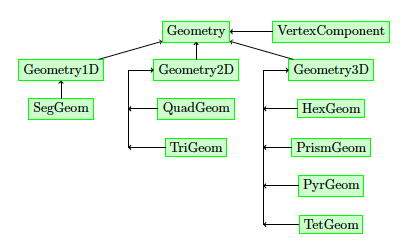
\includegraphics{img/SpatialDomains.png}
\caption{Main classes in the SpatialDomains library.}
\label{f:library:spatialdomains}
\end{figure}


\section{LocalRegions}
The LocalRegions library is designed to encompass all classes that encapsulate
the elemental spectral/hp expansions in physical space, see also the figure
below. It can be appreciated that such a local expansion essentially is a
standard expansion that has a (in C++ parlance) additional coordinate
transformation that maps the standard element to the local element. In an
object-oriented context, these is-a and has-a relationships can be applied as
follows: the classes in the !LocalRegions library are derived from the
{!StdExpansion} class tree but they are supplied with an additional data member
representing the geometry of the local element. Depending on the shape-specific
class in the !LocalRegions library, this additional data member is an object of
the corresponding class in the Geometry class structure. This inheritance
between the !LocalRegions and !StdRegions library also allows for a localised
implementation that prevents code duplication. In order to e.g. evaluate the
integral over a local element, the integrand can be multiplied by the Jacobian
of the coordinate transformation, where after the evaluation is redirected to
the !StdRegions implementation.

This provides extensions of the spectral element formulation into the world. It
provides spatially local forms of the reference space expansions through a
one-to-one linear mapping from a standard straight-sided region to the physical
space, based on the vertices.

\subsection{Local Mappings}

\subsubsection{Linear Mappings}
In one dimension this has the form
\begin{align*}
x = \chi(\xi) = \frac{1-\xi}{2}x_{e-1} + \frac{1+\xi}{2}x_e \quad \xi
\Omega^e
\end{align*}

In two dimensions, for a quadrilateral, each coordinate is given by
\begin{align*}
x_i = \chi(\xi_1,\xi_2) &= x_i^A\frac{1-\xi_1}{2}\frac{1-\xi_2}{2} +
x_i^B\frac{1+\xi_1}{2}\frac{1-\xi_2}{2} \\ &\qquad+
x_i^D\frac{1-\xi_1}{2}\frac{1+\xi_2}{2} +
x_i^C\frac{1+\xi_1}{2}\frac{1+\xi_2}{2}, \quad i=1,2
\end{align*}

\subsubsection{Curvilinear mappings}

The mapping can be extended to curved-sided regions through the use of an
iso-parametric representation. In contrast to the linear mapping, where only
information about the vertices of the element were required, a curvilinear
mapping requires information about the shape of each side. This is provided by
shape functions, $f^A(\xi_1), f^B(\xi_2), f^C(\xi_1)$ and
$f^D(\xi_2)$, in the local coordinate system. For example, the linear
blending function is given by
\begin{align*}
  x_i = \chi_i(\xi_1,\xi_2) &= f^A(\xi_1)\frac{1-\xi_2}{2} +
  f^C(\xi_1)\frac{1+\xi_2}{2} + f^B(\xi_2)\frac{1-\xi_1}{2} +
  f^D(\xi_2)\frac{1+\xi_1}{2}\\ &\qquad-
  \frac{1-\xi_1}{2}\frac{1-\xi_2}{2}f^A(-1) - 
  \frac{1+\xi_1}{2}\frac{1-\xi_2}{2}f^A(1)\\ &\qquad-
  \frac{1-\xi_1}{2}\frac{1+\xi_2}{2}f^C(-1) -
  \frac{1+\xi_1}{2}\frac{1+\xi_2}{2}f^C(1)
\end{align*}

\subsection{Classes}
All local expansions are derived from the top level Expansion base class. Three
classes, Expansion1D, Expansion2D and Expansion3D, are derived from this and
provided base classes for expansions in one-, two- and three- dimensions,
respectively. The various local expansions are derived from these. The class
hierarchy is shown in Figure~\ref{f:library:localregions}.

One dimension:
\begin{itemize}
\item SegExp - Line expansion, local version of StdRegions::StdSegExp.
\end{itemize}

Two dimensions:
\begin{itemize}
\item TriExp - Triangular expansion.
\item QuadExp - Quadrilateral expansion.
\end{itemize}

Three dimensions:
\begin{itemize}
\item TetExp - Tetrehedral expansion. (All triangular faces) 
\item HexExp - Hexahedral expansion. (All rectangular faces)
\item PrismExp - Prism expansion. (Two triangular, three rectangular faces)
\item PyrExp - Pyramid expansion. (One rectangular, four triangular faces)
\end{itemize}

Other classes:
\begin{itemize}
\item PointExp
\item LinSys
\item MatrixKey
\end{itemize}

\begin{figure}
\centering
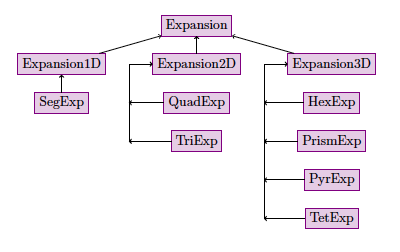
\includegraphics[width=\textwidth]{img/LocalRegions.png}
\caption{Main classes in the LocalRegions library.}
\label{f:library:localregions}
\end{figure}

\section{MultiRegions}
In the MultiRegions library, all classes and routines are related to the
process of assembling a global spectral/hp expansion out of local elemental
contributions are bundled together. The most important entities of this library
are the base class ExpList and its daughter classes. These classes all are the
abstraction of a multi-elemental spectral/hp element expansion. Three different
types of multi-elemental expansions can be distinguished:

\subsection{A collection of local expansions}
This collection is just a list of local expansions, without any coupling between
the expansions on the different elements, and can be formulated as:
\begin{align*}
u^{\delta}(\boldsymbol{x})=\sum_{e=1}^{{N_{\mathrm{el}}}}\sum_{n=0}^{N^{e}_m-1}\hat{u}_n^e\phi_n^e(\boldsymbol{x})
\end{align*}
where
\begin{itemize}
\item ${N_{\mathrm{el}}}$ is the number of elements, 
\item $N^{e}_m$ is the number of local expansion modes within the
element $e$, 
\item $\phi_n^e(\boldsymbol{x})$ is the $n^{th}$ local expansion mode within
the element $e$, 
\item $\hat{u}_n^e$ is the $n^{th}$ local expansion coefficient 
\item within the element $e$.
\end{itemize}

These types of expansion are represented by the classes ExpList0D, ExpList1D,
ExpList2D and ExpList3D, depending on the dimension of the problem (ExpList0D is
used just to deal with boundary conditions for 1D expansions).

\subsection{A multi-elemental discontinuous global expansion}
The expansions are represented by the classes DisContField1D, DisContField2D and
DisContField3D. Objects of these classes should be used when solving partial
differential equations using a discontinuous Galerkin approach. These classes
enforce a coupling between elements and augment the domain with boundary
conditions.

All local elemental expansions are now connected to form a global spectral/hp
representation. This type of global expansion can be defined as:
\begin{align*}
u^{\delta}(\boldsymbol{x})=\sum_{n=0}^{N_{\mathrm{dof}}-1}\hat{u}_n
  \Phi_n(\boldsymbol{x})=\sum_{e=1}^{{N_{\mathrm{el}}}}
  \sum_{n=0}^{N^{e}_m-1}\hat{u}_n^e\phi_n^e(\boldsymbol{x})
\end{align*}
where
\begin{itemize}
\item $N_{\mathrm{dof}}$ refers to the number of global modes, 
\item $\Phi_n(\boldsymbol{x})$ is the $n^{th}$ global
expansion mode, 
\item $\hat{u}_n$ is the $n^{th}$ global expansion coefficient.
\end{itemize}

Typically, a mapping array to relate the global degrees of freedom
$\hat{u}_n$ and local degrees of freedom $\hat{u}_n^e$ is
required to assemble the global expansion out of the local contributions.

In order to solve (second-order) partial differential equations, information
 about the boundary conditions should be incorporated in the expansion. In case
 of a standard Galerkin implementation, the Dirichlet boundary conditions can be
 enforced by lifting a known solution satisfying these conditions, leaving a
 homogeneous Dirichlet problem to be solved. If we denote the unknown solution
 by $u^{\mathcal{H}}(\boldsymbol{x})$ and the known Dirichlet
 boundary conditions by $u^{\mathcal{D}}(\boldsymbol{x})$ then we can
 decompose the solution $u^{\delta}(\boldsymbol{x})$ into the form
\begin{align*}
  u^{\delta}(\boldsymbol{x}_i)=u^{\mathcal{D}}(\boldsymbol{x}_i)+
  u^{\mathcal{H}}(\boldsymbol{x}_i)=\sum_{n=0}^{N^{\mathcal{D}}-1}
  \hat{u}_n^{\mathcal{D}}\Phi_n(\boldsymbol{x}_i)+
  \sum_{n={N^{\mathcal{D}}}}^{N_{\mathrm{dof}}-1}
  \hat{u}_n^{\mathcal{H}}\Phi_n(\boldsymbol{x}_i).
\end{align*}
Implementation-wise, the known solution can be lifted by ordering the known
degrees of freedom $\hat{u}_n^{\mathcal{H}}$ first in the global
solution array $\boldsymbol{\hat{u}}$.


\subsection{A multi-elemental continuous global expansion}
The discontinuous case is supplimented with a global continuity condition. In
this case a $C^0$ continuity condition is imposed across the element
interfaces and the expansion is therefore globally continuous.

This type of global continuous expansion which incorporates the boundary
 conditions are represented by the classes ContField1D, ContField2D and
 ContField3D. Objects of these classes should be used when solving partial
 differential equations using a standard Galerkin approach.


\subsection{Additional classes}
Furthermore, we have two more sets of classes:
\begin{itemize}
\item The class LocalToGlobalBaseMap and its daughter classes:
  LocalToGlobalC0ContMap and LocalToGlobalDGMap.
  
  These classes are an abstraction of the mapping from local to global degrees
  of freedom and contain one or both of the following mapping arrays:
  \begin{itemize}
  \item map $[e][n]$

    This array contains the index of the global degree of freedom corresponding
    to the $n^{th}$ local expansion mode within the $e^{th}$ element.
  \item bmap $[e][n]$
  
    This array contains the index of the global degree of freedom corresponding
    to the $n^{th}$ local boundary mode within the
    $e^{th}$ element.
  \end{itemize}
  Next to the mapping array, these classes also contain routines to assemble the
  global system from the local contributions, and other routines to transform
  between local and global level.
\item The classes GlobalLinSys and GlobalLinSysKey.

  The class GlobalLinSys is an abstraction of the global system matrix
  resulting from the global assembly procedure. Depending of the choice to
  statically condense the global matrix or not, the relevant blocks are stored
  as a member of this class. Given a proper right hand side vector, this class
  also contains a routine to solve the resulting matrix system.
  
  The class GlobalLinSysKey represents a key which uniquely defines a global
  matrix. This key can be used to construct or retrieve the global matrix 
  associated to a certain key.
\end{itemize}

More information about the implementation of connectivity between elements in
Nektar++ can be found [wiki:Connectivity here].

\begin{center}
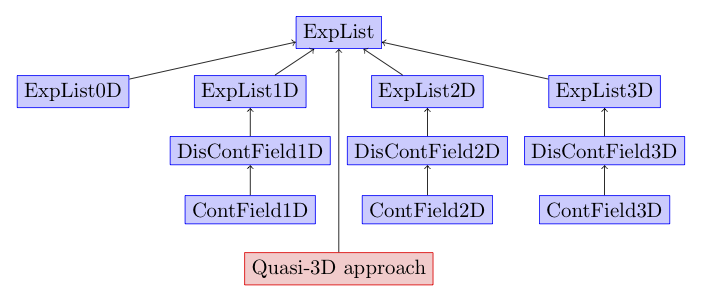
\includegraphics{img/MultiRegions.png}
\end{center}

\subsection{Quasi-3D approach}

The Quasi-3D approach is an extension of the 1D and the 2D spectral/hp element
method. This technique permits to study 3D problems combining the spectral/hp
element method with a spectral method. In the Quasi-3D approach with 1
homogenous direction, the third dimension (z-axis) is expandend with an harmonic
expansion (a Fourier series). In each quadrature point of the Fourier
discretisation we can find a 2D plane discretised with a 2D spectral/hp elements
expasions. In the case with 2 homogeneous directions a plane is discretised with
a 2D Fourier expansion (y-z palne). In each one of the quadrature point of this
harmonic expansion there is a 1D spectral/hp element discretisation. The
homogenous classes derive directly form ExpList, and they are
ExpListHomogeneous1D and ExpListHomogeneous2D. This classes are used to
represent the collections of 2D (or 1D) spectral/hp element problems which are
located in the Fourier expansions quatradure points to create a 3D problem. As
describer above, we can find the find the continuos or discontinuos case,
depending on the spectral/hp element approach. ExpList2DHomogeneous1D and
ExpList1DHomogeneous2D are used to manage boundary conditions. A description of
the Quasi-3D approach usage can be found in Chapter 3 in the User Guide.

\begin{center}
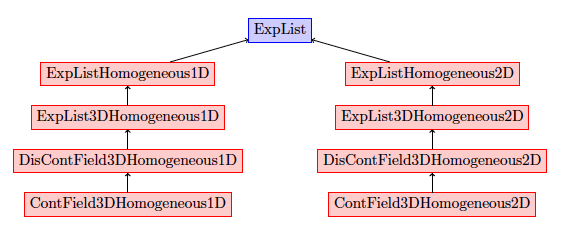
\includegraphics[width=\textwidth]{img/Quasi3d.png}
\end{center}


\section{SolverUtils}

\subsection{Drivers}
Drivers govern the high-level execution of a solver.

\subsubsection{Implementing a new Driver}
To take advantage of the Nektar++ architecture and implement an algorithm 
which will wrap around an existing solver, new drivers can be created. This can
be done in a few steps by using DriverStandard.cpp (and .h) as a template:
\begin{itemize}
\item Create the new files called DriverMyAlgorithm.cpp (and .h)
\item Implement constructor and destructor
\item Provide implementation for \texttt{v\_InitObject} and \texttt{v\_Execute}
as necessary.
\item Register the new driver with the driver factory.
\begin{lstlisting}[style=C++Style]
string DriverMyAlgorithm::className = 
    GetDriverFactory().RegisterCreatorFunction("MyAlgorithm",
                                               DriverMyAlgorithm::create); 
string DriverMyAlgorithm::driverLookupId = 
    LibUtilities::SessionReader::RegisterEnumValue("Driver","MyAlgorithm",0);
\end{lstlisting}
\item Add the new driver to the library. In \inlsh{CMakeLists.txt}, 
DriverMyAlgorithm.cpp must be added in the \inlsh{SOLVER\_UTILS\_SOURCES} 
section and DriverMyAlgorithm.h in the \inlsh{SOLVER\_UTILS\_HEADERS} section.
\end{itemize}